`\chapter{Presenting Data in Figures}

There can be no doubt that the hallmark of scientific reports and publications is the graphical presentation of the results. Graphs show relationships underlying observations in a way no other device can provide\footnote{\textit{Doing science: design, analysis, and communication of scientific research}
 By Ivan Valiela}. 
Charting is both an art and a science. Modern typography on charts and infographics look at Tufte as inspiration.
Tufte advocates to minimize the ink to data ratio and although this is not always possible it is good advice.
In this section we would look at charting in general which is probably of interest to most of the readers
in this book.  Another good source of information is Stephen Few’s website the perceptualedge \footnote{\protect\url{http:\\perceptualedge.com}}  with a number of excellent articles on data visualization. 

\section{Tufte like charts}

During the last stages of a Project, it maybe easier to visualize the
main areas where effort needs to be exerted by using simple charts. One
such chart is shown in Figure~\ref{fig:tufte-overall}. When this chart
was prepared efforts were made to complete the physical installation
as well as plan and commission the plant. The use of colour in this
chart highlights the commissioning, so one can easily see the expectations. Although the percentages are written on top of the bars,
one need not read them to visualize how difficult is to achieve
100\% completion in a Project. On the other hand commissiong can go
fairly fast and can jump by a large percentage, just by
commissioning a couple of additional ELV systems that have approximately
a 10\% weigh factor.

One can easily fit approximately, six to seven months data on
a portrait chart, changing it around to landscape one can fit
more than a year. Personally I am not very happy with such long
projections as they are more like guesses rather than proper estimates.

One other chart that can be used to visualize progress and is more
commonly found in construction is the infamous S-curve. Now, if
the actual planning is detailed enough and granular enough to be
able to pin-point \textit{continuous} progress then it is
appropriate. using it if you can at least obtain weekly progress
estimates.


\begin{figure}[b]
 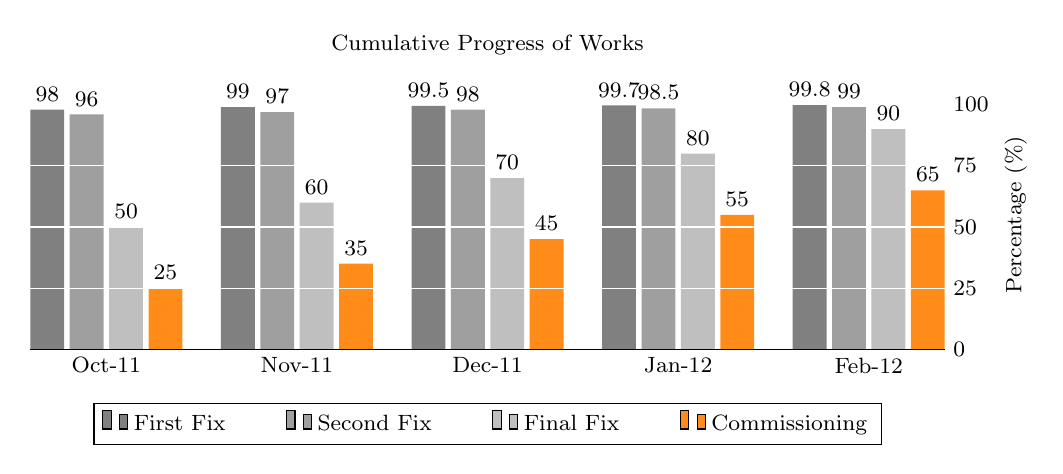
\begin{tikzpicture}
  \footnotesize
  \centering
  \begin{axis}[
        ybar, axis on top,
        title={Cumulative Progress of Works},
        height=5cm, width=13.2cm,
        bar width=0.43cm,
        ymajorgrids, tick align=inside,
        major grid style={draw=white},
        enlarge y limits={value=.1,upper},
        ymin=0, ymax=100,
        axis x line*=bottom,
        axis y line*=right,
        y axis line style={opacity=0},
        ytick={0,25,50,75,100},
        tickwidth=0pt,
        legend style={
            at={(0.5,-0.2)},
            anchor=north,
            legend columns=-1,
            % adds space between the legends
            /tikz/every even column/.append style={column sep=0.7cm}
        },
        ylabel={Percentage (\%)},
        symbolic x coords={
           Sep-11,Oct-11,Nov-11,Dec-11,
           Jan-12,Feb-12,
           Mar-12,
          Apr-12},
       xtick=data,
       nodes near coords={
        \pgfmathprintnumber[precision=2]{\pgfplotspointmeta}
       }
    ]
    \addplot [draw=none, fill=gray] coordinates {
      (Oct-11, 98)
      (Nov-11,99)
      (Dec-11,99.5)
      (Jan-12,99.7)
      (Feb-12,99.8)
       };
   \addplot [draw=none,fill=gray!75!white] coordinates {
      (Oct-11, 96)
      (Nov-11,97)
      (Dec-11,98)
      (Jan-12,98.5)
      (Feb-12,99)
        };
   \addplot [draw=none, fill=gray!50!white] coordinates {
      (Oct-11, 50)
      (Nov-11, 60)
      (Dec-11, 70)
      (Jan-12, 80)
      (Feb-12, 90)
            };
    \addplot [draw=none, fill=orange!90!white] coordinates {
      (Oct-11, 25)
      (Nov-11, 35)
      (Dec-11, 45)
      (Jan-12, 55)
      (Feb-12, 65)
          };
    \legend{First Fix,Second Fix,Final Fix,Commissioning}
  \end{axis}
  \end{tikzpicture}

\caption{\protect\raggedright Cumulative progress for all MEP works. Notice the slower rate of production during the last three months.}
\label{fig:tufte-overall}
\end{figure}

\section{Graph Design}
A good graph is uncluttered, clear and focused.

\subsection{Axis Lines}

Most problems with graphs arise from misuse of axes: too heavy, too long, wrong intersection,
ambiquous breaks or too confusing increments and incorrect proportions. An axis is a ruler that established
regular intervals for measuring the information provided. Axes may emphasize, diminish, distort, simplify
or clutter the information.

\clearpage
\begin{multicols}{2}
\subsection{Axis Length}

Graphs should utilize their space around them, as the graph itself is mostly white space. In publications the journal might want to minimize the cost of printing. An axis should not extend beyond the labeled unit od minor tick closest to the last data point.
\columnbreak
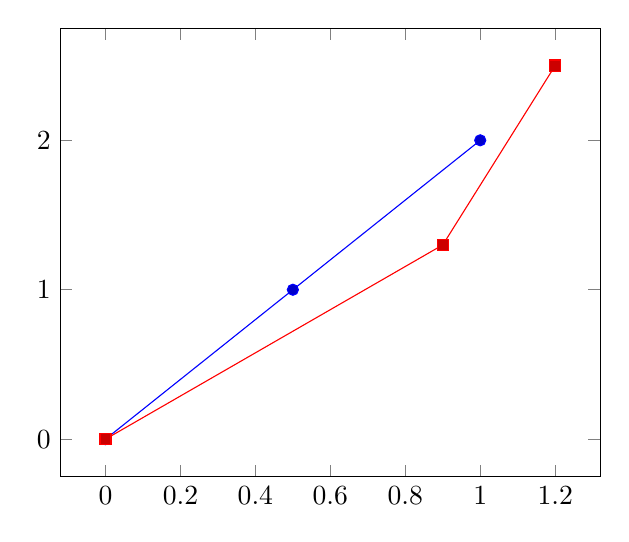
\begin{tikzpicture}
\begin{axis}
\addplot coordinates {
(0,0)
(0.5,1)
(1,2)
};
\addplot coordinates {
(0,0)
(0.9,1.3)
(1.2,2.5)
};
\end{axis}
\end{tikzpicture}
\end{multicols}


\section{The bullet graph}

The bullet graph is considered\footnote{\protect\url{http://www.perceptualedge.com/blog/?p=375}} to be a  better alternative to gauges in dashboards. A solution to a basic chart can be found at tx.se\footnote{\url{http://tex.stackexchange.com/questions/117314/is-there-any-package-to-create-bullet-gauge-graphs}}, by Jake, which sadly in a community of mathematicians, engineers and programmers was not popularized to the extend it deserved. 

Bullet gauges are commonly used to show the current state relative to a reference value with a background that divides the scale into regions.

\begin{figure}[htbp]
\centering

\includegraphics{./images/bullet-graph.png}
\caption{Bullet graph with annotations, indicating the various components of the graph.}
\end{figure}



current sales --
previous sales --
good -- 
great -- last shade box

Formatting: The color is preferable to be a range of distinct hues, which can also assist by those who are colorblind. It is also reproduced better when photocopies.  Intensities are preferred as follows:

three: 40\%, 25\% and 10\%

\makeatletter
\newenvironment {bulletgraph} {\luacode@begin\luacode@table@soft} {}
\makeatother

\pgfplotscreateplotcyclelist{bullet}{
{fill=color1, draw=none},
{fill=color2, draw=none},
{fill=color3, draw=none},
}

\pgfplotsset{mark options/.style={color=black!80}}
\pgfplotsset{barwidth/.style= {bar width=1.2ex} }
\pgfplotsset{chartheight/.style ={height=#1}}

\providecommand{\bulletgauge}[4][]{
    \begin{tikzpicture}[scale=0.8, font=\arial]
    \begin{axis}[
       width=8cm,
       chartheight = 60pt,
      % height=60pt,
       %y=2ex,
       xtick pos=left, 
       xtick = {0,50,...,400, 450},
       ytick=\empty,
       xmin=50, xmax=450,
        %enlarge y limits={abs=0ex},
        tick align=outside,
        axis on top,
        every axis title/.style={
            at={(rel axis cs:0,0.5)},
            anchor=east,
            align=right,
            xshift=-0.5em
        },
        #1
    ]
    \pgfplotsinvokeforeach{#4}{
        \pgfplotsset{cycle list name=bullet}
        \addplot +[xbar, bar width=7ex ] coordinates {(##1,0)};
    }
    \addplot [fill= barcolour, xbar, barwidth ] coordinates {(#2,0)};    
    \addplot [mark=|, mark options={very thick}, mark size=2ex, ] coordinates {(#3,0)}; 
    \end{axis}
    \end{tikzpicture}
}

\begin{scriptexample}{}{}
\begin{bulletgraph}
  m = require("i18n.bulletgraph")
 local data = {
     title = 'Valuation (Jan)',
     ranges = {230,300,500},
     bar = 200,
     marker = 220}
     local options = {
        barcolour = 'red!90'
   } 
m:render(data,options)        
\end{bulletgraph}
\medskip

\begin{bulletgraph}
   m = require("i18n.bulletgraph")
   local data = {
      title = 'Valuation (Apr)',
      ranges = {200,300,500},
      bar = 250,
      marker = 300}
   -- render the plot
   m:render(data,options)           
\end{bulletgraph}
\end{scriptexample}

Use an updated pgfplotsversion as we use |\pgfplotsset{compat=1.11}|, when we load the \pkgname{phd}. The environment |\begin{bulletgraph}|  is a |\luacode|  based environment and hence all the code has to be in lua syntax.

The code load the lua module |bulletgraph| and we the graph is rendered using the method \luacmd{render()}. The method, like most of the plotting routines provided by the package takes two arguments |data| and |options|.

\begin{texexample}{Bullet Plots}{ex:bulletplot}
\begin{bulletgraph}
local  bgraph = require("i18n.bulletgraph")
local data = {
     title = 'Valuation (Jan)',
     ranges = {230,300,500},
     bar = 200,
     marker = 220}
local options = {
        barcolour = 'red!90'
   } 
bgraph:render(data,options)        
\end{bulletgraph}
\end{texexample}

If you are familiar with Javascript you must have come across jQuery and its many plugins. The bulletgraph methods work in a similar fashion, where the options are a set of key values, that are used as a mixin with a set of default key values. If you only want to change the color of the bar, you only specify the color in the options the rest
are inherited from default values. All the \pkgname{phd} package routines, follow this design pattern to simplify the user interface and to enable typographical styles to be maintained throughout a publication. The best way to draw such charts is without the |options|. This separation of the interface, it also separates the data from the presentational aspects of drawing the plots.

\begin{texexample}{Bullet Plots (without options)}{ex:bulletplot1}
\begin{bulletgraph}
local  bgraph = require("i18n.bulletgraph")
local data = {
     title = 'Valuation (Jan)',
     ranges = {230,300,500},
     bar = 200,
     marker = 220}
bgraph:render(data,options)        
\end{bulletgraph}
\end{texexample}













